% Week 6 / Code breaking / Adult guide (F06-FAC-v4)
% Build: ./build.sh  (runs check_guide.py first, which also writes lookup3.tex)
\documentclass[11pt]{article}
\usepackage[letterpaper,top=0.85in,bottom=0.85in,left=0.8in,right=0.8in,
  headheight=14pt,headsep=0.2in,footskip=0.4in]{geometry}
\usepackage[T1]{fontenc}
\usepackage[default]{sourcesanspro}
\usepackage[italic]{mathastext}
\usepackage{microtype}
\usepackage{fancyhdr}
\usepackage[table]{xcolor}
\usepackage{array,tabularx,booktabs}
\usepackage{enumitem}
\usepackage{titlesec}
\usepackage{needspace}
\usepackage{tikz}
\usepackage[most]{tcolorbox}
\usepackage{amsmath}

\setlength{\parindent}{0pt}
\setlength{\parskip}{4pt}
\raggedright

\pagestyle{fancy}
\fancyhf{}
\renewcommand{\headrulewidth}{0pt}
\lhead{\small Week 6 / Code breaking / Adult guide}
\lfoot{\small Bellingham Math Circle / Week 6 / F06-FAC-v4}
\rfoot{\small \thepage}

\titleformat{\section}{\Large\bfseries}{\thesection.}{0.4em}{}
\titlespacing*{\section}{0pt}{10pt}{3pt}
\titleformat{\subsection}{\large\bfseries}{}{0em}{}
\titlespacing*{\subsection}{0pt}{8pt}{2pt}

\setlist{nosep,leftmargin=1.3em,topsep=2pt}
\renewcommand{\arraystretch}{1.15}
\newcolumntype{L}{>{\raggedright\arraybackslash}X}

\newcommand{\cd}[1]{\mbox{\textsf{\textbf{#1}}}}   % a code such as RRY
\definecolor{tagcore}{HTML}{1F5FA8}
\definecolor{tagmore}{HTML}{7A7A7A}
\newcommand{\core}{\textcolor{tagcore}{\textbf{core}}}
\newcommand{\further}{\textcolor{tagmore}{\textbf{further}}}
% \pb{number}{page}{tag}
\newcommand{\pb}[3]{\par\needspace{5\baselineskip}\medskip\textbf{Problem #1}\enspace{\small page #2}\enspace\textperiodcentered\enspace #3\par\nopagebreak}
\newcommand{\lab}[1]{\textbf{#1}\enspace}
\newcommand{\hints}[1]{\lab{Hints}#1}

\tcbset{gbox/.style={breakable,colback=black!4,colframe=black!45,boxrule=0.5pt,arc=2pt,
  left=6pt,right=6pt,top=4pt,bottom=4pt,before skip=6pt,after skip=6pt}}

\begin{document}

\small R = red, Y = yellow. A code such as \cd{RYY} is read from column~1, which is on the breaker's left. A test's \emph{score} is the number of columns where test and secret show the same color. Every answer below was recomputed by \texttt{guide-src/check\_guide.py} from the puzzles and boards in the student sources.
\normalsize

\section{The idea of the week}

Someone hides a thing and you learn about it only from answers. A yes-or-no answer can at best cut what is left in half, so two questions can always pick out one of 4 things, three questions one of 8, four questions one of 16, and never more. In the code game the secret is a row of red-or-yellow counters, and each test row gets a score. A score is an answer with a few possible values. The children find that a code of $n$ counters can always be found with $n$ tests (all red first, then turn over one counter at a time), and the oldest explain why fewer tests cannot always work for 2, 3 and 4 counters. One wrong score makes a game impossible to solve, so scoring is done with objects and every score is checked at the end.

\textbf{A good session looks like this.}
\begin{itemize}
\item \textbf{K--1.} Every child has hidden a block and asked questions, pushing away the blocks that are ruled out. Both pairs have played the two-counter game several times with you scoring, and someone can say why one test is not enough (``red-red got 1, and it could be red-yellow or yellow-red''). Some reach three counters.
\item \textbf{2--3.} Pairs run both games themselves with no scoring mistakes. They have written three questions that always find the block and can say why two cannot (four answer patterns, eight blocks). They break three-counter codes, and the quickest have a method that always takes three tests.
\item \textbf{4--5.} They have written methods that always take 3 tests for three counters and 4 for four, and explained at least one ``cannot'': three questions for 1 to 16, or one test for two counters. The quickest explain why two tests cannot do three counters.
\end{itemize}

\section{Materials and preparation}

\textbf{Counts for this group} (K--1: 2 pairs; 2--3: 2 pairs; 4--5: one pair and a third child).

{\small\begin{tabularx}{\linewidth}{@{}L r r r r@{}}
\toprule
Item, and how many each pair needs & K--1 & 2--3 & 4--5 & Total\\
\midrule
Two-sided counters: K--1 pair 45 (its eight three-counter secrets beside a full board), older pair 30, 4--5 third child 10, plus 10 spare per table. A full board takes 10, 18 or 24 (2, 3, 4 counters). & 100 & 70 & 50 & 220\\
Green pattern-block triangles as scoring tokens, one per column of each board in use, plus 2 spare. Keep them in their own cup. & 8 & 10 & 6 & 24\\
Pattern blocks, one of each of the 8 shapes (a ``set''). Two sets per pair: the picker's set behind a folder, the asker's set to sort. & 4 & 4 & -- & 8 + 1 spare\\
File folders, one per board in use, plus 1 spare & 3 & 3 & 2 & 8\\
Pencils with erasers (children and adult) & 5 & 5 & 4 & 14\\
Small whiteboards and markers & 2 & 2 & 3 & 7\\
\bottomrule
\end{tabularx}}

\medskip
\textbf{Printing.} Single-sided, US Letter, at 100\% (``Actual size'', not ``Fit''): the slots must be 1 inch for a counter, and the triangle outlines must fit a green triangle.

{\small\begin{tabularx}{\linewidth}{@{}l l l L@{}}
\toprule
Packet & Whole packet & Extra board pages & Notes\\
\midrule
K--1, F06-K-v4, 7 pp. & 3 (1 per pair + you) & pp.\,4 and 7: 2 more each & Color for pp.\,1, 2, 5. One page per pair at a time.\\
2--3, F06-M-v4, 10 pp. & 5 (1 per child + you) & pp.\,3, 5, 9: 2 more each & Color for pp.\,1--2. One page at a time.\\
4--5, F06-U-v4, 9 pp. & 4 (1 per child + you) & pp.\,2 and 5: 2 more each & Gray is fine. One page at a time.\\
\bottomrule
\end{tabularx}}

\medskip
\begin{minipage}[t]{0.60\linewidth}
\textbf{Set up every code board page} (K--1 pp.\,4, 7; 2--3 pp.\,3, 5, 9; 4--5 pp.\,2, 5). About 10 minutes in all.
\begin{enumerate}
\item With a pen, write 1, 2, 3 (and 4) above the secret slots, and again above the first test row. Column 1 is the left one as printed.
\item Cut along the dashed ``folder'' line. The top strip (secret, copy of test, triangle outlines) is the \emph{keeper strip}; the bottom strip (test rows, score boxes) is the \emph{breaker strip}. A folder cannot stand on the uncut line.
\item At the table: breaker strip in front of the breaker; a folder opened like a book and stood on its long edges, its point toward the breaker; keeper strip behind it, on the keeper's side.
\item The keeper copies each test \emph{by column number}: test column 1 into copy column 1. This is right whichever way the keeper strip faces. Copying ``left to right'' from across the table reverses the row.
\end{enumerate}
\end{minipage}\hfill
\begin{minipage}[t]{0.36\linewidth}
\vspace{2pt}
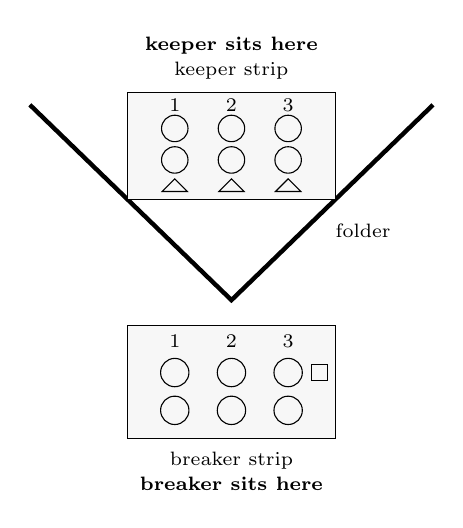
\begin{tikzpicture}[x=0.4cm,y=0.4cm,font=\scriptsize]
  % breaker strip
  \draw[fill=black!3] (-3.3,0) rectangle (3.3,3.6);
  \foreach \x/\n in {-1.8/1,0/2,1.8/3} {\draw (\x,2.1) circle (0.45); \draw (\x,0.9) circle (0.45); \node at (\x,3.1) {\n};}
  \draw (2.55,1.85) rectangle ++(0.5,0.5);
  \node[anchor=north] at (0,-0.1) {breaker strip};
  \node[anchor=north] at (0,-0.9) {\textbf{breaker sits here}};
  % folder: open like a book, standing, point toward the breaker
  \draw[line width=1.6pt] (-6.4,10.6) -- (0,4.4) -- (6.4,10.6);
  \node[anchor=west] at (3.0,6.6) {folder};
  % keeper strip
  \draw[fill=black!3] (-3.3,7.6) rectangle (3.3,11.0);
  \foreach \x/\n in {-1.8/1,0/2,1.8/3} {\draw (\x,9.85) circle (0.42); \draw (\x,8.85) circle (0.42);
     \draw (\x-0.4,7.85) -- (\x+0.4,7.85) -- (\x,8.25) -- cycle; \node at (\x,10.6) {\n};}
  \node[anchor=south] at (0,11.1) {keeper strip};
  \node[anchor=south] at (0,11.9) {\textbf{keeper sits here}};
\end{tikzpicture}
\end{minipage}

\medskip
\textbf{Test with the real materials before the session} (15 minutes, at home).
\begin{itemize}
\item A counter fits inside a printed slot and a green triangle inside a printed outline. If not, the printer shrank the page.
\item The folder stands, and from a seated child's eye height you cannot see the keeper strip.
\item Play one three-counter game against yourself: hide a secret, score three tests by copy-and-triangles, lift the folder, recheck all three scores. The K--1 adult should do this.
\item \textbf{Counter colors.} The pages say red and yellow. If your counters have other colors, decide which side is ``red'' and which is ``yellow'' for this week, put a labeled sticky note under one counter of each in the middle of every table, and say it at the launch: ``On our counters, blue is red and white is yellow.''
\item \textbf{Blocks.} The drawings of the pink right triangle, teal kite and gray dart are approximate; the children use the real blocks. Check the real blocks' colors against the names on the pages. If a color differs, hold up the block at the start and say which name it has today.
\end{itemize}

\section{The hour}

\begin{tabularx}{\linewidth}{@{}l L@{}}
\toprule
0:00--0:05 & Running around.\\
0:05--0:08 & Whole-group launch (organizer): how a test is scored.\\
0:08--0:50 & Tables, about 40 minutes. K--1 and 2--3 start with the blocks; 4--5 starts with the number game.\\
0:50--0:55 & Sharing: one question, each table answers once.\\
\bottomrule
\end{tabularx}

\subsection{Launch (2--3 minutes)}
At the front: a cut two-counter board (an extra copy of 2--3 p.\,3), one folder, 6 counters, 2 green triangles.
\begin{enumerate}
\item Stand the folder. Behind it, put red in column 1 and yellow in column 2. Say: ``Behind the folder is a secret: two counters, each red or yellow.''
\item Say: ``The breaker makes a test: a counter in every slot of the next test row, red or yellow side up.'' One child comes up and fills the first test row. That is a legal move: both slots filled, each counter flat with one color up. An empty slot is not allowed.
\item Say: ``I copy your test under my secret, column 1 into column 1, column 2 into column 2. Where the colors in a column match, I put a green triangle.'' Do it. If the test was red-red: one triangle, under column 1. ``One triangle. Your score is 1.'' The child writes 1 in the score box.
\item Ask the room: ``Which secrets could it be?'' (Red-yellow or yellow-red.) Take the copy and the triangles away. A second child makes the next test; score it the same way.
\item When a child says what the secret is: ``Now I lift the folder, and we check every score again.'' Re-copy each test, recount the triangles aloud, compare with the score box. ``If a check finds a wrong score, that game does not count. We fix it and play again with a new secret.''
\end{enumerate}

\subsection{How each table pairs up}
\begin{itemize}
\item \textbf{K--1, two pairs.} Blocks (Problems 1--4): in each pair one child picks and one asks, then they swap. The picker takes the chosen block from the picker's set and holds it in a closed hand under the table. Stand behind the pickers and check each answer quietly; a wrong answer spoils a round just as a wrong score does. Code games (Problems 6 and 9): you keep the secret and score for both pairs, one board per pair side by side, two folders, you across from both. The two children in a pair take turns building the test and may talk it over. A pair waiting for you works on Problem 5, 7 or 8.
\item \textbf{2--3, two pairs.} In each pair one keeper and one breaker; swap after every game (the new keeper takes the folder and keeper strip). Watch each pair's first two scorings, then look in at every reveal-and-check.
\item \textbf{4--5, a pair and a third child.} Keeper and breaker play; the third child is referee, watches each copy and count, and says ``agreed'' before the score is written. Rotate after each game: keeper to breaker, breaker to referee, referee to keeper. In Problem 1 one child thinks of the number and the other two take turns asking.
\end{itemize}

\subsection{When attention runs out}
\begin{itemize}
\item \textbf{K--1:} hide-a-block. One child hides a real block in a closed hand; the others ask yes-or-no questions; count the questions on your fingers. Or let them build all the secrets of Problem 5 or 8 with counters.
\item \textbf{2--3:} guess my number from 1 to 16 with yes-or-no questions, tallying questions on a whiteboard. Can anyone always do it in 4? (Yes; 3 never always works.)
\item \textbf{4--5:} guess my number from 1 to 100. Is 7 always enough? Is 6? (7 is; 6 is not, because $2^6=64<100$.)
\end{itemize}

\subsection{Sharing question}
\textbf{``With two counters, why can't one test always tell you the secret?''} K--1 answers first. Expected: there are four secrets but only three scores (0, 1, 2); red-red scores 1 for both red-yellow and yellow-red. The 4--5 table may add what they found for three and four counters.

\begin{tcolorbox}[gbox]
\textbf{When a score is wrong (every table).} Signs: the scores fit no secret; the breaker names a secret and the reveal shows another; a child says ``that can't be.''
\begin{enumerate}
\item \textbf{Reveal.} Lift the folder.
\item \textbf{Recheck every score}, from the first test: copy it by column number under the secret, put triangles on the matches, count aloud, compare with the score box.
\item Cross out the wrong score and write the right one. Show which conclusion it broke.
\item \textbf{Replay} with a new secret; the same breaker goes again. The spoiled game does not count.
\end{enumerate}
Usual causes: a test copied in reverse (use the column numbers); triangles left over from the previous test; counting matches against the test row instead of the copy; a counter flipped by a sleeve.
\end{tcolorbox}

\section{Table by table}

\subsection{K--1 table (parent volunteer)}
Read each problem aloud. Core: 1, 2, 3, 5, 6. Further: 4, 7, 8, 9. If a child is struggling, skip Problem 4 and rows 4--5 of Problem 7, and keep playing Problem 6 with new secrets instead of moving to 8 and 9.

\begin{tcolorbox}[gbox]
\textbf{How you score each test (Problems 6 and 9).} You are the keeper; you say only the number.
\begin{enumerate}
\item The child finishes the test row. Check every slot has a counter, red or yellow up.
\item \textbf{Copy:} for column 1, 2, 3, put a counter of the same color in that column of your ``copy of test'' row.
\item \textbf{Match:} in each column where your secret counter and your copy counter show the same color, put a green triangle in that column's triangle outline.
\item \textbf{Count} the triangles aloud. That is the score. The child (or you) writes it in that test row's score box.
\item Clear the copy row and the triangles before the next test.
\end{enumerate}
Things to say: ``Every slot needs a counter.'' ``Which secrets could it still be? Show me with counters.'' ``Are you sure? How do you know?'' ``Say what the secret is; then I lift the folder and we check every score together.''
\end{tcolorbox}

\pb{1}{1}{\core}
One child picks one of the four blocks (triangle, rhombus, trapezoid, hexagon); the other asks yes-or-no questions and pushes away blocks that are ruled out. Put the other four blocks away.\\
\lab{Answer}Yes, two questions always work. Example: ``Does it have four sides?'' Yes leaves rhombus and trapezoid; no leaves triangle and hexagon. Then ask about one of the two left: ``Is it the rhombus?'' Pointing at two blocks, ``Is it one of these two?'', works as a first question too.\\
\hints{(1) ``Ask a question. Which blocks can it not be now? Push them away.'' (2) ``Can you find a question that pushes away two blocks, yes or no?'' (3) Point at two blocks: ``Is it one of these two?''}

\pb{2}{1}{\core}
Only pointing questions: ``Is it this one?''\\
\lab{Answer}7. After seven ``no'' answers one block is left, so you are sure without asking. A child who says 8 has counted asking about the last block; ask ``When one block is left, do you need to ask?''\\
\hints{(1) Play it, pushing away each ``no''. (2) ``What if the secret is the last block you point to?'' (3) ``When one block is left, are you sure?''}

\pb{3}{2}{\core}
All eight blocks, three questions.\\
\lab{Answer}Yes. Each question has to leave half: 8, then 4, then 2, then 1. Example: ``Is it in the top row of the picture?'' (triangle, rhombus, trapezoid, hexagon). ``Does it have four sides?'' Two blocks are left: ``Is it this one?''\\
\hints{(1) ``If the answer to your first question is no, how many blocks are left? If yes?'' (2) ``Find a first question where yes leaves four and no leaves four.'' (3) ``Four blocks took two questions in Problem 1. Can one question take you from eight to four?''}

\pb{4}{2}{\further}
The child picks; the partner may ask only two questions.\\
\lab{Answer}No. With the blocks: ``Whatever the first question is, the yes pile or the no pile has at least four blocks. The second question leaves at least two of those. With two left, you can't be sure.'' Or: two answers make only four patterns (yes-yes, yes-no, no-yes, no-no), and eight blocks on four patterns means two blocks share one.\\
\hints{(1) Play it; after each answer push away the blocks that are out and count what is left. (2) ``If yes leaves three blocks, how many does no leave?'' (3) Lay four sheets of paper for yes-yes, yes-no, no-yes, no-no, and sort the blocks onto them for two questions.}

\pb{5}{3}{\core}
Make every two-counter secret in the trays.\\
\lab{Answer}4: \cd{RR}, \cd{RY}, \cd{YR}, \cd{YY}. Red-yellow and yellow-red are different (the first place differs). Two trays stay empty.\\
\hints{(1) ``Make one secret. Now make one that is different.'' (2) ``Is there another one that starts with red?'' (3) ``Put the ones that start with red together and the ones that start with yellow together.''}

\pb{6}{4}{\core\ (the main game)}
You keep the secret and score; the pair makes tests.\\
\lab{Answer}One test: \textbf{no}. Red-red scores 1 for both red-yellow and yellow-red, and every test has two secrets that score 1. Two tests: \textbf{yes}. Test red-red: 2 means red-red; 0 means yellow-yellow; 1 means red-yellow or yellow-red, so test red-yellow next: 2 means red-yellow, 0 means yellow-red. (After a 1, the second test must have one red and one yellow.) Sometimes one test is enough: red-red scoring 0 or 2.\\
\hints{(1) ``Put the four secrets from Problem 5 next to the board. After each score, push away the ones that could not get that score.'' (2) ``Red-red got 1. Which secrets have just one red?'' (3) ``Try a test with one red and one yellow.''}

\pb{7}{5}{\further}
For each row of drawn tests and scores, put counters on every secret that could be hiding. Each row has two trays.\\
\lab{Answer}Row 1 (\cd{RR} scores 2): \cd{RR}. Row 2 (\cd{RY} scores 0): \cd{YR}. Row 3 (\cd{RR} scores 1): \cd{RY} and \cd{YR}, both trays. Row 4 (\cd{RR} 1, \cd{YR} 0): \cd{RY}. Row 5 (\cd{RY} 1, \cd{RR} 0): \cd{YY}.\\
\hints{(1) ``Take the four secrets from Problem 5. Score this test against each one with triangles.'' (2) ``Score 0 means no place matches: every counter is the other color.'' (3) Two tests: ``Find the secrets that fit the first test, then check those with the second.''}

\pb{8}{6}{\further}
Every three-counter secret in the trays.\\
\lab{Answer}8: \cd{RRR}, \cd{RRY}, \cd{RYR}, \cd{RYY}, \cd{YRR}, \cd{YRY}, \cd{YYR}, \cd{YYY}. Two trays stay empty.\\
\hints{(1) ``Make the four two-counter secrets again and put a red at the end of each.'' (2) ``Now make them again with a yellow at the end.'' (3) ``How many have three reds? Two? One? None?'' (1, 3, 3, 1.)}

\pb{9}{7}{\further}
The same game with three counters.\\
\lab{Answer}Yes, three tests always work. Test 1: all red; the score is the number of reds in the secret. Test 2: all red with only the first counter turned over (\cd{YRR}); if the score goes up by one, the secret's first counter is yellow; if it goes down by one, red. Test 3: \cd{RYR}, the same for the second counter. The third counter is whatever makes the number of reds right. It is enough if someone notices that all red counts the reds.\\
\hints{(1) ``Make the test all red. What does the score tell you?'' (2) ``Now turn over only the first counter and test again. Did the score go up or down?'' (3) ``Up means the first counter of the secret is yellow; down means red.''}

\subsection{2--3 table}
Core: 1--7. Further: 8--11. If a child is struggling, play 3 and 5 without the written explanation, replay 4 and 6 instead of moving on, and skip 9.

\pb{1}{1}{\core}
Block game behind a folder, questions per round in the boxes; then rounds where every question names one block.\\
\lab{Answer}Good questions take 3. Naming one block at a time: at most 7 (the round ends when you are sure; 8 if they also ask about the last block).\\
\hints{(1) ``Which of your questions pushed away the most blocks, whatever the answer?'' (2) Naming rounds: ``What if it is the last block you name?''}

\pb{2}{2}{\core}
Write questions that always find the block in three; test them on a partner.\\
\lab{Answer}Possible. Three fixed questions: Q1 ``Is it the triangle, rhombus, trapezoid or hexagon?'' (top row of the picture), Q2 ``Does it have exactly four sides?'', Q3 ``Is it red, yellow, purple or gray?'' Answer patterns (Y/N): triangle YNN, rhombus YYN, trapezoid YYY, hexagon YNY, chevron NNY, right triangle NNN, kite NYN, dart NYY; all different. Any plan that halves 8, 4, 2 works, including one where the second question depends on the first answer.\\
\hints{(1) ``After your first question, how many blocks are left if yes? If no?'' (2) ``Find a first question that leaves four either way.'' (3) ``For each group of four, find a question that leaves two.''}

\pb{3}{2}{\core}
Decide whether two questions can always be enough, and explain.\\
\lab{Answer}No. Two yes-or-no answers have only four patterns; with eight blocks two share a pattern, and if the secret is one of them you cannot tell. With objects: choose two questions and sort the blocks into four piles (yes-yes, yes-no, no-yes, no-no); some pile has two or more. If the second question depends on the first answer: the first answer leaves at least 4, the second at least 2.\\
\hints{(1) ``Take two questions and sort the eight blocks by their answers.'' (2) ``How many different answer pairs are there?'' (3) ``Eight blocks, four piles: what must happen?''}

\pb{4}{3}{\core}
Two-counter game in pairs.\\
\lab{Answer}Two tests always suffice (\cd{RR}; after a score of 1, \cd{RY}); one test is enough when \cd{RR} scores 0 or 2.\\
\hints{(1) ``Which secrets fit this score? Build them.'' (2) ``Which second test gives those different scores?''}

\pb{5}{4}{\core}
Try one-test and two-test plans in the record tables; explain.\\
\lab{Answer}One test: no. A test has three possible scores (0, 1, 2) and there are four secrets; concretely, the two rows you get by turning over one counter of the test both score 1. Two tests: yes, as in Problem 4; even the fixed pair \cd{RR}, \cd{RY} works: \cd{RR}\,(2,1), \cd{RY}\,(1,2), \cd{YR}\,(1,0), \cd{YY}\,(0,1).\\
\hints{(1) ``Build a test. Which secrets would give it a 1?'' (2) ``How many different scores can one test get? How many secrets are there?''}

\pb{6}{5}{\core}
Three-counter game.\\
\lab{Answer}Three tests always suffice (method in Problem 8); two can never always (4--5 Problem 8).\\
\hints{(1) ``What does an all-red test tell you?'' (2) ``Change one counter and test again. What does the change in the score tell you?''}

\pb{7}{6}{\core}
Write every three-counter secret that fits each finished game.\\
\lab{Answer}Game 1 (\cd{RRR} 2): \cd{RRY}, \cd{RYR}, \cd{YRR}. Game 2 (\cd{RYR} 1, \cd{YYR} 2): \cd{YRR}, \cd{YYY}. Game 3 (\cd{RYY} 2, \cd{YRY} 2, \cd{RRR} 2): \cd{RRY}; each row alone leaves three, so all three are needed. Game 4 (\cd{RRY} 2, \cd{RYR} 2, \cd{YRR} 2): \cd{RRR}. Game 5 (\cd{RRR} 3, \cd{RYR} 1): none. \cd{RRR} scoring 3 means the secret is \cd{RRR}, and then \cd{RYR} would score 2: the keeper made a scoring mistake.\\
\hints{(1) ``Lay out all eight secrets and score the first test against each.'' (2) ``A score of 2 out of 3 means exactly one place is wrong.'' (3) ``Keep the ones that fit, then check them with the next test.''}

\pb{8}{7}{\further}
\begin{minipage}[t]{0.66\linewidth}
Write a three-counter method someone else could follow.\\
\lab{Answer}\cd{RRR}, then \cd{YRR}, then \cd{RYR}. The first score $r$ is the number of reds. The second is $r+1$ if the first counter is yellow, $r-1$ if red; the third does the same for the second counter. The third counter makes the number of reds equal to $r$. The table gives all eight score triples; they are all different, so the three tests can even be fixed in advance.\\
\hints{(1) ``What does the all-red score tell you?'' (2) ``Turn over one counter and test again: by how much can the score change?'' (3) ``Do you need a test for the last counter?''}
\end{minipage}\hfill
\begin{minipage}[t]{0.3\linewidth}\vspace{0pt}\small
% generated by check_guide.py
\begin{tabular}{@{}l ccc@{}}\toprule
Secret & \cd{RRR} & \cd{YRR} & \cd{RYR} \\\midrule
\cd{RRR} & 3 & 2 & 2 \\
\cd{RRY} & 2 & 1 & 1 \\
\cd{RYR} & 2 & 1 & 3 \\
\cd{YRR} & 2 & 3 & 1 \\
\cd{RYY} & 1 & 0 & 2 \\
\cd{YRY} & 1 & 2 & 0 \\
\cd{YYR} & 1 & 2 & 2 \\
\cd{YYY} & 0 & 1 & 1 \\
\bottomrule\end{tabular}

\end{minipage}

\pb{9}{8}{\further}
Play games that end only when a test scores 3; explain.\\
\lab{Answer}Yes. With Problem 8's method you know the secret after three tests; the fourth test is the secret itself and scores 3 (or an earlier test already scored 3). Ending by the third test cannot be promised; that needs the argument of 4--5 Problem 8 and is not asked here.\\
\hints{(1) ``After three tests of your method, what do you know?'' (2) ``What should the fourth test be?''}

\pb{10}{9}{\further}
Four-counter game.\\
\lab{Answer}Four tests always suffice; three never always (4--5 Problem 9).\\
\hints{(1) ``Start all red. What do you learn?'' (2) ``Change one counter at a time. Do you need a test for the last one?''}

\pb{11}{10}{\further}
Write a four-counter method and its worst case.\\
\lab{Answer}\cd{RRRR}, \cd{YRRR}, \cd{RYRR}, \cd{RRYR}; the fourth counter from the number of reds: at most 4 tests. Testing every place separately without the count takes 5. No method can always use 3 (computer check; proof in 4--5 Problem 9); do not press this here.\\
\hints{(1) ``Does your three-counter method work with one more counter?'' (2) ``Do you need a test for the last place?''}

\subsection{4--5 table (organizer)}
Core: 1--6. Further: 7--10. If a child is struggling, drop games 4--5 of Problem 3, and do Problem 7 (one experiment) before attempting 8.

\pb{1}{1}{\core}
Guess-my-number by yes-or-no questions, 1 to 16 and then 1 to 20; explain the lower bound.\\
\lab{Answer}1 to 16: 4 questions (halve each time: ``more than 8?'', and so on). Fewer: three questions give $2\cdot2\cdot2=8$ answer patterns for 16 numbers, so two numbers share a pattern. 1 to 20: 5. Four questions give 16 patterns, fewer than 20; five suffice ($20\to10\to5\to3\to2\to1$).\\
\hints{(1) ``Which question cuts the numbers in half?'' (2) ``Write down every answer pattern three questions can give. How many are there?''}

\pb{2}{2}{\core}
Three-counter games, rotating keeper, breaker and referee.\\
\lab{Answer}Three tests always suffice; two never always (Problem 8).\\
\hints{(1) ``What does an all-red test tell you?'' (2) ``Turn over one counter and test again. What does the change in the score tell you?'' (3) ``Do you need a test for the last counter?''}

\pb{3}{3}{\core}
Find every secret that fits each finished game, three and four counters.\\
\lab{Answer}Game 1: \cd{RRR}. Game 2 (\cd{RRR} 2, \cd{RYY} 2): \cd{RRY}, \cd{RYR}. Game 3 (\cd{RRYY} 3, \cd{YRYR} 1, \cd{RRRY} 2): \cd{RYYY}. Game 4 (\cd{RRYY} 2, \cd{RYRY} 2, \cd{RYYR} 2): \cd{RRRR} and \cd{YYYY}. Game 5 (\cd{RYRY} 1, \cd{RRYY} 3, \cd{YYYY} 2): none, a scoring mistake. Child's reason: \cd{RRYY} and \cd{YYYY} differ in exactly two places, and changing two counters of a test changes its score by 0 or 2, never by 1; but 3 and 2 differ by 1. (Adult view: all three tests have an even number of Y, so all three scores have the parity of the number of Y in the secret; 1, 3, 2 are not all of one parity.)\\
\hints{(1) ``A score of 3 out of 4 means one place is wrong. Which secrets are those?'' (2) ``Check each of them against the other tests.'' (3) Game 5: ``Compare \cd{RRYY} and \cd{YYYY}. How much can the score change when you change two counters?''}

\pb{4}{4}{\core}
Write a three-counter method that always works in three tests.\\
\lab{Answer}As 2--3 Problem 8: \cd{RRR}, \cd{YRR}, \cd{RYR}; the last counter from the count. Score table in the 2--3 section.\\
\hints{(1) ``Look at a game you won in three tests. What did the first test tell you?'' (2) ``If you change one counter between tests, what can the score change tell you?''}

\pb{5}{5}{\core}
Four-counter games.\\
\lab{Answer}Four tests always suffice; three never always (Problem 9).\\
\hints{(1) ``Start all red. What do you learn?'' (2) ``Can your three-counter method work here?''}

\pb{6}{6}{\core}
Write a four-counter method that always works in four tests.\\
\lab{Answer}\cd{RRRR}, \cd{YRRR}, \cd{RYRR}, \cd{RRYR}; each score after the first is one more (yellow) or one less (red) than the first; the fourth counter from the count.\\
\hints{(1) ``Does your three-counter method stretch?'' (2) ``Do you need to test the last place?''}

\pb{7}{7}{\further}
Score a secret row against a test row, turn over both counters in one place, score again.\\
\lab{Answer}The score does not change, for any rows and any place. Child's reason: in that place, two counters that matched still match after both are turned over (red-red becomes yellow-yellow), and two that did not match still do not; the other places are untouched. Use: you may always pretend the first test is all red.\\
\hints{(1) ``Try it with three different pairs of rows and different places.'' (2) ``Look only at the place you turned over. Did those two counters match before? After?''}

\pb{8}{7}{\further}
Explain two impossibilities: one test for two counters, two tests for three.\\
\lab{Answer}One test, two counters: three scores, four secrets; the two rows one turn away from the test both score 1.
Two tests, three counters (counting does not help: $4\cdot4=16\ge 8$): take the three rows you get by turning over one counter of test 1. Each scores 2 on test 1, so the breaker cannot tell them apart and faces them with the same test 2. Turning over one counter changes a row's score on any other test by exactly 1. So on test 2 each of the three scores (test 2's score against the test-1 row) plus or minus 1: two values for three secrets. With counters: lay out test 1, the three one-turn rows, any test 2, and score.\\
\hints{(1) ``Which secrets score 2 on your first test?'' (2) ``Turn over one counter of a row. How much can its score on another test change?''}

\pb{9}{8}{\further}
Decide whether three tests can do four counters; explain.\\
\lab{Answer}No. Take the six rows with two counters of test 1 turned over; each scores 2 on test 1. For any later test $T$, let $s$ be $T$'s score against the test-1 row and $D$ the places where $T$ differs from test 1. A row turned at places $Q$ scores $s-2+2|Q\cap D|$: only three values. As $|D|=0,1,2,3,4$, test 2 splits the six as 6; 3+3; 1+4+1; 3+3; 6, so a group of 3 or 4 is left. Test 3 gives a group of four at most three values. A group of three is either the three pairs containing one fixed place or the three pairs inside three places, and test 3 gives either at most two values. So two secrets always share all three scores (also checked by computer). A child can see the start: ``any test gives the six only three scores, and never two, two and two.''\\
\hints{(1) ``Which secrets score 2 on your first test? How many?'' (2) ``Try a second test on all six. How do they split?''}

\pb{10}{9}{\further}
Games that end only on a full score, three and four counters; explain both answers. The four-counter board has four test rows, so a fifth test goes in a record table on the page.\\
\lab{Answer}Three counters: 4. Four counters: 5. Enough: know the secret after $n$ tests (Problems 4, 6), then test it. Not fewer: suppose a way always ended by test $n$. After $n-1$ tests either some test scored $n$, or the $n$-th test (fixed by the scores so far) must be the secret. Either way the first $n-1$ scores already tell the secret, contradicting Problems 8 and 9.\\
\hints{(1) ``After your method's tests, what do you know? What should the next test be?'' (2) ``Suppose some way always ended by test 3 with three counters. What would you know after test 2?'' (3) ``What did Problem 8 say about two tests?''}

\section{The mathematics behind the week}

\textbf{Counting answers.} If each answer has at most $m$ possible values, $k$ answers have at most $m^k$ patterns, so they can be sure of separating at most $m^k$ things. For yes-or-no questions this is $2^k$, and halving reaches it, so $N$ things need exactly $\lceil\log_2 N\rceil$ questions: 3 for 8 blocks, 4 for 16, 5 for 20, 7 for 100. Letting a question depend on earlier answers does not help: a decision tree of depth $k$ has at most $2^k$ leaves (the same bound gives $\log_2 n!$ comparisons for sorting).

\textbf{The code game.} Secrets are $s\in\{R,Y\}^n$ and the score of a test $t$ is $n-d(t,s)$, with $d$ the Hamming distance. Turning over the same places in test and secret preserves $d$, so every score is unchanged (4--5 Problem 7); hence the first test may be taken to be all red, and its score is the number of reds.
\begin{itemize}
\item \emph{$n$ tests suffice}: all red, then all red with place $i$ turned over for $i=1,\dots,n-1$; each moves the score by $\pm1$, which gives color $i$, and the last color comes from the count. These tests can be fixed in advance.
\item \emph{Counting is too weak}: a test has $n+1$ scores, and $(n+1)^k\ge 2^n$ only forces $k\ge2$ for $n=2,3,4$. The true minimum (exhaustive adaptive search) is 2, 3, 4 for $n=2,3,4$. The proofs use the neighbors of the first test: the $n$ one-turn neighbors all score $n-1$ and any later test gives them only two values (enough for $n=3$); for $n=4$ the six two-turn neighbors need the finer count in 4--5 Problem 9.
\item \emph{Ending on a full score} costs exactly one more test: 3, 4, 5. A strategy that always ends by test $k$ knows the secret after $k-1$ tests.
\item \emph{Parity}: $d(t,s)\equiv w(t)+w(s) \pmod 2$, where $w$ counts yellows, so tests with the same parity of yellows give scores of one parity. This catches some scoring errors (4--5 Problem 3, game 5).
\end{itemize}

\textbf{Where it goes next.} Five counters already need only 4 tests; for instance the fixed tests \cd{RRRRR}, \cd{RRRYY}, \cd{RRYRY}, \cd{RYRRY} give all 32 secrets different scores. Once the number of reds is known, a test's score says how many of the test's yellow places are yellow in the secret, which is a spring-scale weighing of a set of coins. This is the coin-weighing problem of Erdős and Rényi (1963): for long codes far fewer than $n$ tests suffice, on the order of $n/\log n$; with tests fixed in advance about $2n/\log_2 n$ are needed and suffice (Lindström; Cantor and Mills). Mastermind with 4 places and 6 colors and two kinds of score can always be solved in 5 guesses (Knuth, 1976). Natural next sessions: three colors; a balance scale, whose three outcomes give $3^k$ (12 coins, one fake, 3 weighings); twenty questions.

\section{What to write down after the session}

For each table, a few lines:
\begin{itemize}
\item Problems reached by each pair (circle the numbers on your copy).
\item What children tried and said, with first names: a question they asked, a wrong idea, a method in their own words.
\item One drawing or claim worth keeping: a photo of a finished board, a written method, a list of secrets.
\item Games spoiled by a wrong score, and the cause.
\item For each claim below that a child made, its status: \textbf{T} tried (played it), \textbf{G} guessed, \textbf{C} checked in some cases, \textbf{E} explained.
\end{itemize}

{\small\renewcommand{\arraystretch}{1.55}
\begin{tabularx}{\linewidth}{@{}L l p{0.8in} p{0.45in} p{1.45in}@{}}
\toprule
Claim & Table & Who & Status & Words used\\
\midrule
Two questions always find one of 4 blocks & K--1 & & & \\
\arrayrulecolor{black!25}\midrule[0.3pt]\arrayrulecolor{black}
Pointing only can need 7 questions & K--1, 2--3 & & & \\
\arrayrulecolor{black!25}\midrule[0.3pt]\arrayrulecolor{black}
Three questions always find one of 8 blocks; two cannot & K--1, 2--3 & & & \\
\arrayrulecolor{black!25}\midrule[0.3pt]\arrayrulecolor{black}
There are 4 two-counter and 8 three-counter secrets & K--1 & & & \\
\arrayrulecolor{black!25}\midrule[0.3pt]\arrayrulecolor{black}
One test is not enough for two counters; two tests are & all & & & \\
\arrayrulecolor{black!25}\midrule[0.3pt]\arrayrulecolor{black}
All red counts the reds; turning one counter moves the score by 1 & all & & & \\
\arrayrulecolor{black!25}\midrule[0.3pt]\arrayrulecolor{black}
Three tests for three counters, four for four & 2--3, 4--5 & & & \\
\arrayrulecolor{black!25}\midrule[0.3pt]\arrayrulecolor{black}
Two tests cannot do three counters; three cannot do four & 4--5 & & & \\
\arrayrulecolor{black!25}\midrule[0.3pt]\arrayrulecolor{black}
Ending on a full score takes one more test & 2--3, 4--5 & & & \\
\arrayrulecolor{black!25}\midrule[0.3pt]\arrayrulecolor{black}
A game that fits no secret means a scoring mistake & 2--3, 4--5 & & & \\
\arrayrulecolor{black!25}\midrule[0.3pt]\arrayrulecolor{black}
1 to 16 takes 4 questions; 1 to 20 takes 5 & 4--5 & & & \\
\bottomrule
\end{tabularx}}

\end{document}
